\documentclass[11pt]{article}
\usepackage{geometry}                
\geometry{letterpaper}                   

\usepackage{graphicx}
\usepackage{amssymb}
\usepackage{epstopdf}
\usepackage{natbib}
\usepackage{amssymb, amsmath}
\DeclareGraphicsRule{.tif}{png}{.png}{`convert #1 `dirname #1`/`basename #1 .tif`.png}

%\title{Title}
%\author{Name 1, Name 2}
%\date{date} 

\begin{document}



\thispagestyle{empty}

\begin{center}

\includegraphics[width=5cm]{ETHlogo.eps}

\bigskip


\bigskip


\bigskip


\LARGE{ 	Lecture with Computer Exercises:\\ }
\LARGE{ Modelling and Simulating Social Systems with MATLAB\\}

\bigskip

\bigskip

\small{Project Report}\\

\bigskip

\bigskip

\bigskip

\bigskip


\begin{tabular}{|c|}
\hline
\\
\textbf{\LARGE{Civil Violence: Modelling Genocides}}\\
\textbf{\LARGE{Model Extension and Global Sensitivity Analysis}}\\
\\
\hline
\end{tabular}
\bigskip

\bigskip

\bigskip

\LARGE{Ruben W\"alchli \& Zoran Bjelobrk}



\bigskip

\bigskip

\bigskip

\bigskip

\bigskip

\bigskip

\bigskip

\bigskip

Zurich\\
\today\\

\end{center}



\newpage

%%%%%%%%%%%%%%%%%%%%%%%%%%%%%%%%%%%%%%%%%%%%%%%%%

\newpage
\section*{Agreement for free-download}
\bigskip


\bigskip


\large We hereby agree to make our source code for this project freely available for download from the web pages of the SOMS chair. Furthermore, we assure that all source code is written by ourselves and is not violating any copyright restrictions.

\begin{center}

\bigskip


\bigskip


\begin{tabular}{@{}p{3.3cm}@{}p{6cm}@{}@{}p{6cm}@{}}
\begin{minipage}{3cm}

\end{minipage}
&
\begin{minipage}{6cm}
\vspace{2mm} \large Ruben W\"alchli

 \vspace{\baselineskip}

\end{minipage}
&
\begin{minipage}{6cm}

\large Zoran Bjelobrk

\end{minipage}
\end{tabular}


\end{center}
\newpage

%%%%%%%%%%%%%%%%%%%%%%%%%%%%%%%%%%%%%%%



% IMPORTANT
% you MUST include the ETH declaration of originality here; it is available for download on the course website or at http://www.ethz.ch/faculty/exams/plagiarism/index_EN; it can be printed as pdf and should be filled out in handwriting


%%%%%%%%%% Table of content %%%%%%%%%%%%%%%%%

\tableofcontents

\newpage

%%%%%%%%%%%%%%%%%%%%%%%%%%%%%%%%%%%%%%%



\section{Abstract}
A agent-based model for describing an artificial society consisting out of civilians of two different ethnic groups and law enforcement officers (LEOs) was implemented in MATLAB. The model was modified by changing the nature of two characteristic quantities of the civilians, the perceived legitimacy $L$ of the other ethnic group and the violence threshold $T$, making them individual characteristics of the civilians, heterogeneous across the population. Further, a new interaction describing the update of the perceived legitimacy of the other civilians whenever a civilian is killed or arrested was introduced. This modified model was implemented as well in MATLAB.\\
\\
For both model, was tried to quantify the effects of the various input parameters by using a variance-based global sensitivity analysis method. The goal was to identify the most influential parameters for both models and to then describe their effect on the model output. The two models should then have been compared based on those findings. However, the global sensitivity analysis failed by giving senseless values for the sensitivity indices. This was potentially due to a insufficient size of the input parameter samples necessary to compute the indices.\\
\\
The effects of some model parameters on the outputs of the two models were then assessed in a more qualitative manner. The variations of the characteristics $L$ and $T$ over the population introduce more violence compared to otherwise identical situations in the base model. This is due to the presence of few extreme individuals in the society. In reality, in any society there are also extreme individuals, who will very likely commit violence under many circumstances. The parameter $k_L$ seems to have no significant influence on the model output in the current version of the modified model. This may change, when the nature of the interaction is further modified. In general, it appears to be logical, that the perceived legitimacy will be affected by events in the society.

\section{Individual contributions}
Zoran: drinking coffee, meeting girls, playing with latex, etc.

\section{Introduction and Motivations}
Ethnical conflicts were omnipresent throughout human history and still are a major source for civil violence in these days. The wars leading to the decay of former Yugoslavia are an example in the recent past. When studying the project suggestions, this topic immediately drew our interest.\\
\\
Our project is a so-called "model-driven" project. The base model was described by Epstein in 2002. It contains some very strong simplifications as further described in section \ref{subsec:base_model}. Our approach was to modify the model in a way that describes reality better in our opinion and to compare the results of the modified model runs to those of the base model presented in literature. To further assess the models in a quantitative manner, it was tried to perform a global sensitivity analysis for most of the model parameters based on a method described in literature.\\
\\
The main questions of this work were: Is it possible to relax some of the assumptions made in literature and introduce new interactions to make the model more realistic? Can the effects of the model parameters on the outcome of the simulation be quantified, both for the base and the modified model? Having identified the most influential parameters, what is the dependence of the simulation outcomes on them? Can in the end, based on those results, a statement be made about the qualitative and quantitative difference between the base and the modified model? Does the modified model actually describe the reality better than the base model?

\section{Description of the Model}
\label{sec:description_model}

\subsection{Base Model}
\label{subsec:base_model}
The model is a so-called agent-based model. There are two fundamental classes of agents: civilians and law enforcement officers (LEOs). The only purpose of the LEOs is to prevent violence through arresting active, this means violent, civilians. The civilians are further divided into two ethnical groups. They become active or stay quiet (peaceful) based on the values of their individual characteristics and the environment within their range of sight. The agents are placed on a two-dimensional map on which they can move and interact with each other.

\subsubsection{Specification of the Civilians}
The will of a civilian to become violent is described by its grievance $G$. This individual grievance is described by two components: the hardship $H$ of the civilian and his perceived legitimacy of the other ethnic group $L$.
\begin{align}
G = H (1 - L)
\end{align}
The grievance of the individual civilian is according to this formula given by the hardship multiplied by the "illegitimacy" $(1 - L)$ of the other ethnic group. The hardship is heterogeneous across the civilians. It is initialized for each civilian at the beginning of the simulation by drawing it from the uniform distribution on the interval $[0,1]$ ($U(0,1)$) and it remains constant over the course of the simulation. $L$ is homogeneous across all civilians and also stays constant. It is also equal for both ethnic groups. It is defined at the beginning of the simulation and also lies between 0 and 1.\\
\\
$R$ is the risk aversion of the civilian. It is heterogeneous across the population and also drawn upon initialization from $U(0,1)$. A civilian inspects his environment before deciding whether to go active or stay quiet (and vice versa). The civilians have the vision $v$, which is homogeneous across the population and is defined at the beginning of the simulation. $P$ is the arrest probability estimated by the civilian.
\begin{align}
P = 1 - \exp \left( - k_P \left( \frac{LEO}{A} \right)_v \right)
\end{align}
$\left(LEO/A\right)_v$ is the LEO-to-active ratio within the civilians vision. $A$ is always at least $1$, because the civilian counts himself as active when calculating the arrest probability. The reasoning behind this calculation is, that it is less likely for the civilian to be arrested, when already a lot of other civilians are acting violently and very few LEOs are present around him. The opposite can be said, if there are a lot of LEOs and only few or no active civilians. $k_P$ is a constant parameter, its value was calculated in literature by setting $P = 0.9$ when $\left(LEO/A\right)_v = 1$. With the risk aversion and the estimated arrest probability the so-called net risk of the civilian of going active can be calculated:
\begin{align}
N = RP
\end{align}
The difference $G - N$ is the civilian's net utility of becoming active. This is compared to a threshold value $T$. If $(G - N) > T$ the civilian becomes or stays active and if $(G - N) \leq T$ the civilian stays or becomes quiet. The threshold value $T$ is equal for all civilians and defined at the beginning of the simulation.

\subsubsection{Specification of the LEOs}
The LEOs have only one characteristic, their vision $v^\star$. They inspect the map within their vision and randomly arrest an active civilian.

\subsubsection{Evolution of the Simulation}
After choosing values for the global parameters, the three different types of agents are placed on the map randomly and their individual attributes are initialized. The number of civilians and LEOs that are placed on the map are determined by their corresponding selected densities. Each iteration begins by the random selection of one agent (civilian or LEO). This agent moves to a random empty position within his vision. There he inspects his environment. If the agent is a civilian he takes the decision to be active or quiet. When he decides to become active, he tries to kill a random civilian of the other ethnic group within his vision. If the selected agent is a LEO, he arrests a random active civilian within his vision. The arrested civilian is assigned a jail term and moved to the jail. The jail term is drawn from $U(0,J_{\text{max}})$. The ages both of the civilians on the map as well as of those in jail are updated and the civilians that have reached their maximum age are removed. The number of turns of the inmates spent in jail are updated and those who have served their time are released onto random positions on the map.

\subsection{Modification of the Model}

\subsubsection{Individual Perceived Legitimacy and Threshold}
In our opinion, the assumption that the perceived legitimacy of the other ethnic group and the threshold value are identical for all individuals of the population is too harsh. Therefore, we wanted to make them individual quantities. To us it also seemed not realistic to have the perceived legitimacy uniformly distributed throughout the population. Therefore, we decided to use the Gaussian distribution truncated to the interval $[0,1]$. In the modified model the perceived legitimacy of the other ethnic group is initialized for all civilians by drawing it from this distribution. This adds two parameters to the model: the mean $\mu_L$ and the standard deviation $\sigma_L$ of the legitimacy.\\
\\
The threshold $T$ can be seen as the level of "extremism" an individual has. Epstein describes it as the utility of not publicly expressing one's private grievance. A very extreme individual will see absolutely no utility in holding his private grievance back, whether a very conservative individual will almost never publicly express his private grievance. The difference $(G-N)$ on the other hand is the perceived utility to express one's private grievance publicly and it can take values in the interval $[-1,1]$. A civilian with $T = -1$ will always be active, whereas a civilian with $T = 1$ will never be active. As said before, it is probably unrealistic to have the threshold value uniformly distributed over the population. Therefore, it is also drawn upon initialization of the civilians from the truncated Gaussian distribution on the interval $[-1,1]$ adding another two parameters to the model, $\mu_T$ and $\sigma_T$.\\
\\
For the sake of simplicity and to make the sensitivity analysis described later computationally not too expensive, it is renounced to also change the uniform distributions of the other individual characteristics of the civilians ($H$ and $R$) to truncated Gaussian distributions.

\subsubsection{Updating the Perceived Legitimacy}
It seems quite obvious that the perceived legitimacy of the other ethnic group should not be a constant over the course of the simulation. Violence committed by one ethnic group will probably decrease its perceived legitimacy in the eyes of the other ethnic group. The opposite effect will possibly have the arrest of an active (violent) civilian on the perceived legitimacy of its ethnic group. In our expansion of the model, these effects are limited to the range of sight of the involved killed or arrested active civilian. The update in the case of violence is the following:
\begin{align}
L_{\text{new}} = L_{\text{old}} \left( 1 - k_L \right)
\label{eqn:update_violence}
\end{align}
Violence is assumed to have always the same effect on the perceived legitimacy. People are assumed to take violence in general invariably serious no matter the current level of perceived legitimacy. When an active civilian is arrested, the update is given by:
\begin{align}
L_{\text{new}} = L_{\text{old}} + k_L \left( 1 - L_{\text{old}} \right) L_{\text{old}}
\label{eqn:update_arrest}
\end{align}
The reasoning behind the second formula is that if the perceived legitimacy is either very high or very low, arrests only change little in the legitimacy (saturation effect). On the other hand, when a civilian is unsure about the legitimacy of the other ethnic group, arrests are supposed to have a strong influence.

\subsection{Global Sensitivity Analysis of Model Parameters}
In order to test the sensitivity of the output of a generic model with respect to its inputs, a variance-based global sensitivity analysis can be performed as proposed in literature. For the sake of simplicity, we restrict ourselves to scalar model outputs. Most generally speaking, the model is a arbitrary relation $Y = f(X_1,X_2,...,X_k)$ between the output variable $Y$ and the $k$ input variables (parameters) $X_i$. Variance-based sensitivity analysis methods provide quantitative measures how the variance of the output depends on different uncertain/random inputs. Those measures can be interpreted as quantities describing the influence of those inputs on the model output in general. The main advantages of variance-based global sensitivity analysis techniques are their abilities to describe the influence of each input parameter over its full range of values and to detect interactions between the input parameters. Their main disadvantage is their computational cost.\\
\\
For each input parameter $X_i$, a first-order sensitivity index $S_i$ and total-effect index $S_{T_i}$ can be defined:
\begin{align}
S_i &= \frac{V[E(Y|X_i)]}{V(Y)} \label{eqn:first_order}\\
S_{T_i} &= \frac{E[V(Y|\textbf{X}_{\sim i})]}{V(Y)} = 1 - \frac{V[E(Y|\textbf{X}_{\sim i})]}{V(Y)} \label{eqn:total_effect}
\end{align}
$V(Y)$ is the unconditional variance of $Y$, $E(Y|X_i)$ the expectation value of $Y$ conditioned on $X_i$ and $V[E(Y|X_i)]$ the variance of the conditional expectation (fixed/known value of $X_i$). This is measure for sensitivity to changes in the parameter $X_i$. After normalization to the unconditional variance $V(Y)$ one obtains the first-order sensitivity index, which is also called the main effect of $X_i$.\\
\\
$V[E(Y|\textbf{Y}_{\sim i})]$ on the other hand is the output variance $V(Y)$ conditioned on all input variables except $X_i$, i.e. $\textbf{X}_{\sim i}$. This is the remaining variance of the expectation value, if the true values of all input parameters except $X_i$ would be known.\\
\\
The values both of $S_i$ and of $S_{T_i}$ have to be by definition between 0 and 1 as well as  $S_{T_i}$ has to be larger or equal to $S_i$. The bigger $S_i$ and $S_{T_i}$ are, the higher is the effect of the input variable $X_i$ onto the output variable $Y$. The difference $(S_{T_i} - S_i)$ provides information on how much $X_i$ interferes with the other input parameters. If it is zero, there are no interactions. For a purely additive model is $\sum_{i=1}^k S_i = 1$. The difference $1 - \sum_{i=1}^k S_i$ gives a general measure of the amount of interactions in the model.\\
\\
The conditional variances (e.g. $V[E(Y|X_i)]$) can be calculated with a Monte Carlo method using randomly generated sets of input parameters and the corresponding outputs of the model. The implementation is described in section \ref{sec:imp_SA}. Further information about this method of global sensitivity analysis can be found in the literature.

\subsection{Qualitative Assessment of the Input Parameters}
Unfortunately, the global sensitivity analysis yielded no useful results. Therefore, an alternative had to be found in order to assess the influence of certain input parameters on the simulation outcomes and in the end discuss the differences between the two models. The focus was put on the changed procedures and the newly introduced interaction as well as the comparison of the two models with each other.

\section{Implementation}
The whole implementation is based on arrays of structs. This way of implementation may not be the fastest possible, but it is in our opinion the most intuitive one.

\subsection{Base Model}
The fields of the struct used to describe the agents are shown in table \ref{tab:fields_struct}. The central part of the program is the map, an array of size $(N_{\text{map}} \times N_{\text{map}})$ containing this struct as entries, where $N$ is the map size. The individual values of the fields are initialized at the beginning using the function $fun\_init\_map()$, which returns the initialized map array with all the civilians and LEOs. Type equal to 1, 2 or 3 indicates that the agent is a civilian of the ethnic group 1, group 2 or a LEO. For a LEO only the field v is also different from the default value.
\begin{table}[!htbp]
	\centering
	\caption{The fields of the struct used to describe the single agents and their meaning and default value.}
	\vspace{0.5 cm}
		\begin{tabular}{l | l | l} 
			Field Name & Quantity & Default Value\\
			\hline
			type & Type of the Agent & 0\\
			H & Agent's Hardship & 0\\
			L & Agent's Perceived Legitimacy & 0\\
			v & Agent's Vision & 0\\
			T & Agent's Violence Threshold & 0\\
			R & Agent's Risk Aversion & 0\\
			state & Agent's State & 0\\
			age & Agent's Age & 0\\
			life\_exp & Agent's Life Expectancy & 0\\
			sentenced & Agent's Jail Term & 0\\
			served & Agent's Served Time in Jail & 0
	\end{tabular}
	\label{tab:fields_struct}
\end{table}
The jail is an array of size $(J_{max} \times 1)$ with the struct from table \ref{tab:fields_struct} as entries. The reasoning behind the size of the jail array is that it has to be large enough that theoretically in every iteration a civilian could be send to jail. The function $fun\_movement()$ moves the randomly selected agent, updates the map accordingly and returns the new position of the agent. The agents cannot penetrate the borders of the map. If the selected agent is a LEO, the function $fun\_action\_LEO()$ inspects the fields within vision of the new position and if active civilians are present there, randomly moves one of them to the jail. To do so, it first assigns the civilian a random jail term (field "sentenced"). Then copies the civilians struct entries to an empty position in the jail and erases the civilian from the map by setting the struct fields at its position to the default values.\\
\\
If the selected and moved agent is a civilian, the function $fun\_action\_civ()$ is called. It first inspects the surrounding of the new position and determines the current value of $P$ and with this the net risk $N$. The grievance $G$ is also computed and it is checked if $(G-N)$ is larger or smaller than $T$. If it is larger, civilians of the other ethnic group within vision are searched. When there is one present, he is killed by setting all the values of the struct at his position to the default values. If there is no such civilian present, the agent remains quiet although he wants to become active. If $(G-N)$ is smaller than $T$, the selected civilian remains or becomes quiet in any case. The state of the selected civilian remains unchanged, when $(G-N) > T$, but no adversarial civilian is within his vision.The function returns the changed map and if there has been a kill.\\
\\
After moving the agent and performing his action, the function $fun\_clone()$ is called. It goes through all civilians on the map in a random order. For each civilian it checks, if there are empty position right next to him. When there is an empty position, the civilian is cloned with probability $P_c$ onto this position by copying the struct of the selected civilian. The age of the newly created civilian is reset to 0.\\
\\
The $fun\_update\_map()$ function updates the ages of the civilians on the map and removes those who have reached their life expectancy by resetting the struct on those positions to the default one.\\
\\
The jail is updated using the function $fun\_update\_jail()$. First it updates the ages and the served times of the civilians in jail, then it removes civilians that have reached their life expectancy and releases the civilians that have served their sentence onto random empty positions on the map. The structs of those civilians in the jail array are reset to the default values. The civilians are released in the quiet state, all other characteristics remain unchanged.

\subsection{Modified Model}

\subsubsection{Heterogeneity of the Parameters $L$ and $T$}
The function $truncate()$ is used in order to obtain two truncated probability density objects. The normal probability density objects are first created with the desired mean and standard deviation using the function $makedist()$. So in the case of the modified model, the function $fun\_init\_map()$ takes instead of the two parameters $L$ and $T$ the four parameters $\mu_L$, $\sigma_L$, $\mu_T$ and $\sigma_T$. The function $random()$ is then used to initialize the individual values of $L$ and $T$ of the civilians from the truncated normal probability density objects.

\subsubsection{Update of the Perceived Legitimacy}
The function $fun\_action\_civ()$ of the modified model records the position and the ethnic group of the possible killed civilian. Then it inspects the neighborhood within vision of the killed civilian and records the civilians of the same ethnic group. Their perceived legitimacy is then updated according to equation \eqref{eqn:update_violence}. The update described in equation~\eqref{eqn:update_arrest} is incorporated similarly in the function $fun\_action\_LEO()$ of the modified model.

\subsection{Global Sensitivity Analysis}
\label{sec:imp_SA}
For both models, the output variable describing the extent of violence that occurred during the simulation was defined as the cumulative number of kills divided by the initial population size. The normalization to the population size was done in order to investigate the initial population density as input parameter of the models as well. The parameters investigated and their corresponding intervals $[a_i,b_i]$ are shown in table \ref{tab:parameter_intervals}. The remaining model parameters, whose impact on the model output were not investigated are the maximum age of the civilians and the size of the map $N_{\text{map}}$. They were set to 200 and 40, respectively. They both should not qualitatively change the results of the global sensitivity analysis. The number of model iterations used to generate the output was also set to 200. A higher number would have prohibitively increased the computational cost of the analysis. Therefore, we decided to investigate the artificial society for the duration of one generation of civilians. This should however enable us to make a statement about the sensitivity of the occurring violence towards the different parameters.\\
\\
The initial population density $\rho_\textrm{tot}$ was varied between the extremes of a unpopulated and a densely populated map. The fraction $\chi_1$ of the first ethnic group of the population of civilians was varied between the extremes of being a strong minority and being the vast majority. The LEO/civilian ratio gives the ratio between law enforcement officers and civilians. This parameters was varied between having no and having strong law enforcement. A value larger than 0.1 seems to be unrealistic even in authoritarian states. The probability $P_c$ of the civilians to clone themselves in one iteration was not set to 0 because this would lead to a dying out of the entire population in any case. Setting it higher than 0.05 would lead to a unrealistically fast population of the entire map. The range of the visions both of the civilians and the LEOs were obtained in a reasonable relation to the map size. The parameter $k_P$ was varied around the value reported in literature. For $k_P = 1$, the estimated probability of a civilian to be arrested when there are no other active civilians present within vision is $\approx$60\% and for $k_P = 3$ it is $\approx$95\%. The maximum jail term was varied between a very mild and a lifelong sentence. The (mean) perceived legitimacy and violence threshold were varied almost over their entire possible range. Even more extreme values seemed not very sensible, since the outcome of the simulation would be obvious. The standard deviations $\sigma_L$ and $\sigma_T$ of the truncated normal distributions from which the individual values of $L$ and $T$ are initialized in the case of the modified model were varied from the case of a very sharp to a almost uniform distribution over the respective range of possible values. The values of the parameter $k_L$ of the modified model were varied over the entire possible range of values.
\begin{table}[!htbp]
\centering
\caption{Model input parameters and their investigated ranges in the global sensitivity analysis, both for the base and the modified model.}
\vspace{0.5 cm}
	\begin{tabular}{l l l l | l l l l}
	\multicolumn{4}{ c |}{\textbf{Base Model}} & \multicolumn{4}{c}{\textbf{Modified Model}}       \\
	Nr. & $X_i$   & $a_i$ & $b_i$   & Nr. & $X_i$ & $a_i$ & $b_i$ \\ \hline
	1 & $\rho_\textrm{tot}$ & 0.1 & 0.9 & 1 & $\rho_\textrm{tot}$ & 0.1 & 0.9\\ 
	2 & $\chi_1$                      &   0.1    &   0.9   & 2 & $\chi_1$  &   0.1    &   0.9   \\
	3 & LEO/civilian &   0    &   0.1   & 3 & LEO/civilian &   0    &   0.1 \\
	4 & $P_c$ &   0.001    &   0.05  & 4 & $P_c$ &   0.001    &   0.05 \\
	5 & $v$      &   1    &  5   & 5 & $v$      &   1    &  5  \\
	6 & $v^\star$      &   1    &   5   & 6 & $v^\star$      &   1    &   5    \\
	7 &$k_\mathrm{P}$  &   1    &   3  & 7 & $k_\mathrm{P}$  &   1    &   3 \\
	8 & $J_\mathrm{max}$      &   10    &   200   & 8 & $J_\mathrm{max}$ & 10 & 200 \\
	9 & $L$ &   0.1    &   0.9   & 9 & $\mu_L$ & 0.1 & 0.9\\
	 &      &       &      & 10 &  $\sigma_L$ & 0.05 & 1\\
	 10 & $T$ &  -0.9   &   0.9   & 11 & $\mu_T$ & -0.9 & 0.9 \\
	 &       &       &      & 12 & $\sigma_T$ & 0.05 & 1\\
	 &      &       &      & 13 &  $k_L$ & 0 & 1\\
	\end{tabular}
	\label{tab:parameter_intervals}
\end{table}


\subsubsection{Sample Generation}
The size $N$ of the base sample generated was 100. The necessary $(N \times 2k)$ base sample matrix of random numbers, where $k$ is the number of parameters investigated, was generated as suggested in the literature using the sobolset class, which is an implementation of Sobol's random number generator in MATLAB. The procedure to obtain the matrix from a created point set object of this class was directly taken from the documentation of the software. This matrix was divided as described in literature into the two matrices $\boldsymbol{A}$ and $\boldsymbol{B}$, which in turn were used to construct the $k$ matrices $\boldsymbol{C_i}$. The matrix $\boldsymbol{C_i}$ corresponds to the generic parameter $i$ and contains all columns of $\boldsymbol{B}$ except the $i^{\text{th}}$, which is taken from the $i^{\text{th}}$ column of $\boldsymbol{A}$. The sample generation was done inside the program $sample\_generation$ and the created sample matrices were exported into .txt files.

\subsubsection{Model Output Generation}
The implemented models were integrated each into a function called $fun\_model()$ which takes the defined input parameters as arguments and returns the normalized cumulative number of kills. This function was used to generate the output values corresponding to the sets of input parameters contained in the rows of the matrices $\boldsymbol{A}$, $\boldsymbol{B}$ and $\boldsymbol{C_i}$. Sobol's quasi-random number generator produces numbers between 0 and 1. Therefore, the input parameters had to be converted inside the functions $fun\_model()$ in order have their values in the desired ranges. This was done using interval mapping, which is shortly illustrated here:
\begin{align*}
& X_i^\prime \in [0,1] \longmapsto X_i \in [a_i,b_i]\\
&X_i = (b_i-a_i) \cdot X_i^\prime + a_i
\end{align*}
For input parameters that should take integer values ($v$, $v^\star$ and $J_\mathrm{max}$), the MATLAB function $round()$ was used. The interval $[a_i,b_i]$ was extended by 0.5 on both ends for those parameters in order not to increase the probability of having the parameter values $a_i$ and $b_i$ to the same level of the other values in the interval. The output values were stored in the $(N \times 1)$ vectors $\boldsymbol{y_A}$, $\boldsymbol{y_B}$ and $\boldsymbol{y_{C_i}}$. All of this was done inside the program $output\_generation$.

\subsubsection{Sensitivity Indices Computation}
$S_i$ and $S_{T_i}$ were computed with using the generated model outputs $\boldsymbol{y_A}$, $\boldsymbol{y_B}$ and $\boldsymbol{y_{C_i}}$. The unconditional variance of the model output was computed as
\begin{align}
V(Y) = \frac{1}{N} \sum_{j = 1}^N {\left( y_A^{(j)} \right)}^2 - \left( \frac{1}{N} \sum_{j = 1}^N y_A^{(j)} \right)^2
\end{align}
The first term on the right-hand side is the estimate of $E(Y^2)$ and the second term is the estimate of $E(Y)^2$. The conditional variance $V[E(Y|X_i)]$ was calculated as
\begin{align}
V[E(Y|X_i)] = \frac{1}{N} \sum_{j = 1}^N y_A^{(j)} y_{C_i}^{(j)} - \left( \frac{1}{N} \sum_{j = 1}^N y_A^{(j)} \right)^2
\end{align}
and the other necessary conditional variance $V[E(Y|\textbf{X}_{\sim i})]$ was calculated as
\begin{align}
V[E(Y|\textbf{X}_{\sim i})] = \frac{1}{N} \sum_{j = 1}^N y_B^{(j)} y_{C_i}^{(j)} - \left( \frac{1}{N} \sum_{j = 1}^N y_A^{(j)} \right)^2
\end{align}
The first-order sensitivity and the total-effect indices were then calculated according to equations~\eqref{eqn:first_order} and \eqref{eqn:total_effect}.

\subsection{Qualitative Assessment of the Input Parameters}
After the global sensitivity analysis failed by yielding no sensible results, a more qualitative approach was taken to nevertheless be able to discuss the effect of certain input parameters on the simulation outcome, both of the base and the modified model. In the frame of the following analyses it was renounced to normalize the cumulative number of kills to the initial population size, because this parameter was never varied. The output variable of the models was directly the cumulative number of kills.

\subsubsection{Reproduction of Literature Results}
It was tried to reproduce the observations made in literature using the base model. The first reported observation is that peaceful coexistence (with or without LEOs) only prevails, when the perceived legitimacy is very high, i. e. $\geq 0.9$. When the legitimacy is slightly lower (e.g. 0.8) violence starts to break out. The presence of LEOs can prevent the complete extinction of one ethnic group, but not the omnipresence of ethnic violence. $T$/$\mu_T$ was set to 0.1 for the test of this finding. The values of the other model parameters are shown in table~\ref{tab:values_parameters}.
\begin{table}[!htbp]
	\centering
	\caption{}
	\vspace{0.5 cm}
		\begin{tabular}{l | l}
		Parameter & Value\\
		\hline
		$N_{\text{map}}$ & 40\\
		Max. Age & 200\\
		$\rho_{\text{tot}}$ & 0.7\\
		$\chi_1$ & 0.5\\
		$P_c$ & 0.025\\
		$v$ & 2\\
		$v^\star$ & 3\\
		$k_P$ & 2.3\\
		$J_{\text{max}}$ & 30\\
		Number of Iterations & 200\\
	\end{tabular}
	\label{tab:values_parameters}
\end{table}
\\
\\
The second reported observation is regarding the dependence of the time it takes until the extinction of one group on the LEO density on the map. In the literature, the number of iterations was set to 15'000 and for each value of the initial LEO density the simulation was run 50 times. If no extinction happened, after 15'000 iteration the simulation was interrupted. The mean extinction time is reported to increase with increasing LEO density, whereat its standard deviation also increases. The procedure presented in literature was not exactly reproduced. In our opinion, it is not a very good way to assess the violence during the simulation. Very violent conflicts can never lead to the extinction of one ethnic group, but to very high number of casualties. Also this method was no feasible for us, given our computational resources.\\
\\
Therefore, we again decided to let the simulation run for one generation of civilians. The initial LEO/civilian ratio was varied from 0 to 0.1 in steps of 0.004. $L$/$\mu_L$ was set to 0.8 and $T$/$\mu_T$ to 0.1. $\sigma_L$ and $\sigma_T$ were both set to 0.1 in order to have moderately broad distributions. $k_L$ was set to 0.1 for a moderate effect of kills/arrests on the perceived legitimacy. The model was run 10 times at each input parameter value. The mean and the standard deviation of the output variables were taken.\\
\\
An other minor difference to the reference is the selection of the LEO density. In the reference model, the LEO density on the map can be set independently from the population density of the civilians. In our implementation of the model, only the initial LEO/civilian ratio can be selected. This was mainly done in order to prevent situations where there are too many agents to be placed on the map upon initialization. However, this leads only to minor differences, the general trends should not be affected by this.

\subsubsection{Dependence on the Legitimacy and the Violence Threshold}
The dependence on the values of the perceived legitimacy and the violence threshold was evaluated by simultaneously varying $L$/$\mu_L$ and $T$/$\mu_T$ in the range of $[0,1]$ and $[-1,1]$, respectively. For each combination of values, the simulation was run 10 times and the mean and the standard deviation of the resulting model outputs were computed. The LEO/civilian ratio was set to 0.05 and $\sigma_L$/$\sigma_T$ were again set to 0.1. $k_L$ was set to 0.1. The values of all the other model/simulation parameters were taken from table~\ref{tab:values_parameters}.

\subsubsection{Dependence on the Parameters $\sigma_L$ and $\sigma_T$}
For the modified model also the dependence of the model output on the standard deviations of the truncated normal distributions used to initialize the individual values of $L$ and $T$ of the civilians was investigated. For the sake of simplicity, it was assumed that they both take the same value. The LEO/civilian ratio and the means $\mu_L$ and $\mu_T$ as well as the parameter $k_L$ were set to the same values as in the previous section. The other parameter values were again taken from table~\ref{tab:values_parameters}. 

\subsubsection{Dependence on the Parameter $k_L$}
To finish the qualitative analysis, it was also tried to assess the dependence of the extent of violence in the simulation on the parameter $k_L$. Its value was varied in the range of $[0,1]$. Again, $\mu_L$ was set to 0.8, $\mu_T$ to 0.1, the LEO/civilian ratio to 0.05 and $\sigma_L$/$\sigma_T$ to 0.1.

\section{Simulation Results and Discussion}

\subsection{Global Sensitivity Analysis}
The computed sensitivity indices of the input parameters of the base and the modified model are presented in table~\ref{tab:val_sen_ind}, respectively. It is right away obvious that those values cannot be correct. For instance, the $S_i$ have to take by definition values in the interval $[0,1]$ and the sum of the $S_i$ has to be equal to 1. Also, $S_i^T$ has to be larger or equal to $S_i$. To our knowledge, we have made no mistake in the implementation of the global sensitivity analysis in MATLAB. One possible explanation for the failure could be an insufficiently large base sample, leading to inaccurate estimates of the sensitivity indices. But it goes past our computational resources to increase the sample size significantly in order to check, if that is actually the case.
\begin{table}[!htbp]
	\centering
	\caption{Sensitivity indices computed for the input parameters of both models. The meaning of the parameter numbering is explained in table~\ref{tab:parameter_intervals}.}
	\vspace{0.5 cm}
		\begin{tabular}{c | c | c | c | c}
		 & \multicolumn{2}{ c |}{\textbf{Base Model}} & \multicolumn{2}{c}{\textbf{Modified Model}}\\
		Parameter & $S_i$ & $S_i^T$ & $S_i$ & $S_i^T$\\
		\hline
		1 & 0.4748 & 0.2421 & 0.3993 & 1.0651\\
		2 & -0.0147 & -0.7522 & -0.1700 & 0.7317\\
		3 & 0.0464 & -1.0529 & -0.2336 & 0.8763\\
		4 & 0.0360 & -1.1220 & -0.1632 & 0.7517\\
		5 & 0.0810 & -1.1282 & -0.1535 & 0.7772\\
		6 & 0.0640 & -1.1080 & -0.1971 & 0.7879\\
		7 & 0.0559 & -1.1037 & -0.1700 & 0.7482\\
		8 & 0.0765 & -1.0351 & -0.2087 & 0.8419\\
		9 & 0.3150 & -0.0658 & -0.2013 & 0.7784\\
		10 & 0.1213 & -0.9992 & -0.2031 & 0.8355\\
		11 & - & - & -0.0380 & 0.9466\\
		12 & - & - & -0.1666 & 0.8387\\
		13 & - & - & -0.1948 & 0.7765
	\end{tabular}
	\label{tab:val_sen_ind}
\end{table}

\subsection{Qualitative Assessment of the Input Parameters}

\subsubsection{Reproduction of Literature Results}
The result of the analysis regarding the initial LEO/civilian ratio is shown in figure \label{fig:LEO_civ_base}. The anticipated dependence of the mean cumulative number of kills on the LEO/civilian ratio was observed. However, the standard deviation did not increase as one might expect from the results presented in literature. This might be due to the different violence measure used or the effect of the initial LEO/civilian ratio on the standard deviation might only manifest itself at larger numbers of iterations. Also the smaller number of runs per parameter value might affect the result.
\begin{figure}[!htbp]
	\centering
		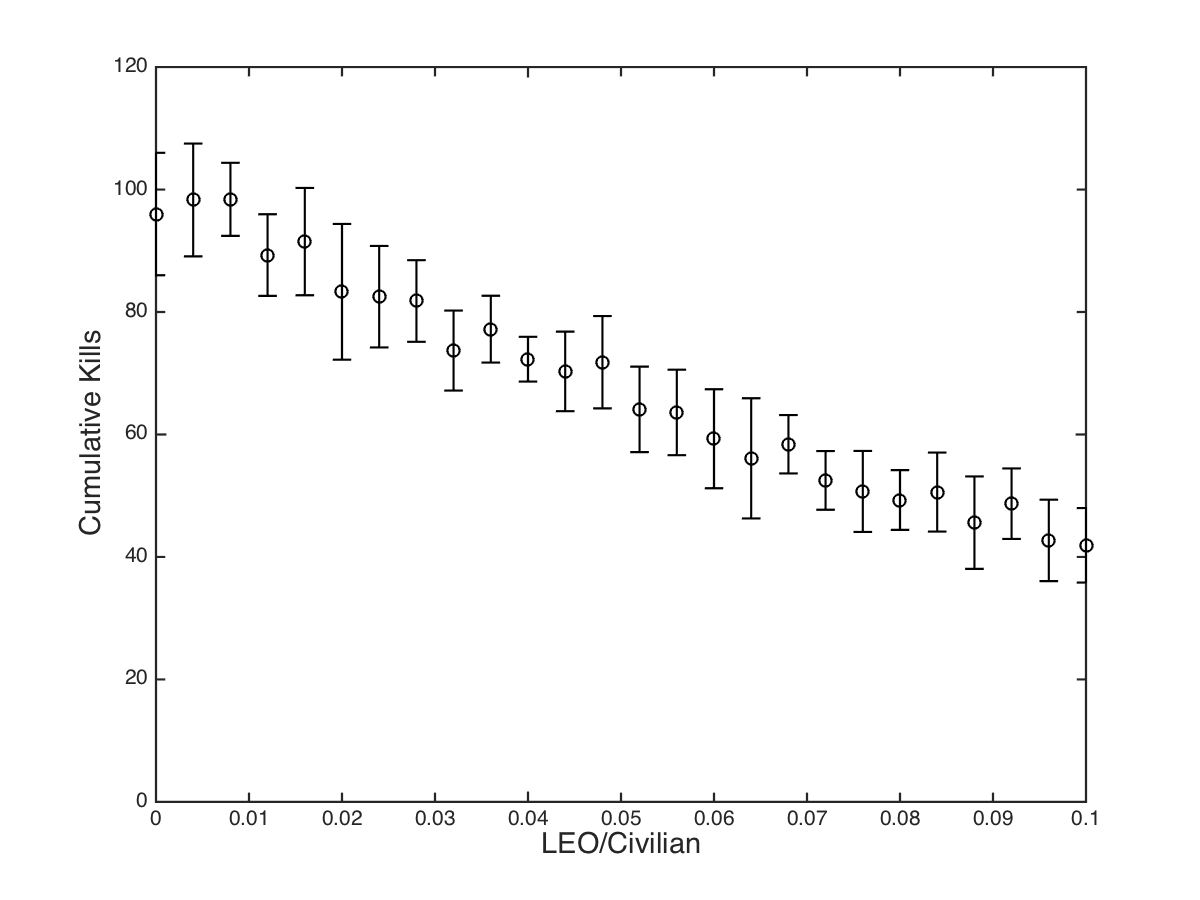
\includegraphics[width=0.80\textwidth]{../../code/base_model/cum_kills_vs_LEO_civ.png}
	\caption{Effect of the initial LEO/civilian ratio on the cumulative number of kills at the end of the simulation using the base model. As expected, the mean formed out of 10 runs decreases with increasing LEO/civilian ratio. The standard deviation on the other hand remains constant. It is shown via the error bars.}
	\label{fig:LEO_civ_base}
\end{figure}
The result of the similar analysis done for the modified model is shown in figure \ref{fig:LEO_civ_modified}. It does not differ from that using the base model. This implies that the heterogeneity of the perceived legitimacy and the violence threshold as well as the updating of the legitimacy has no effect on the dependency of the cumulative number of kills on the initial LEO/civilian ratio, at least not at those values of all the other parameters. 
\begin{figure}[!htbp]
	\centering
		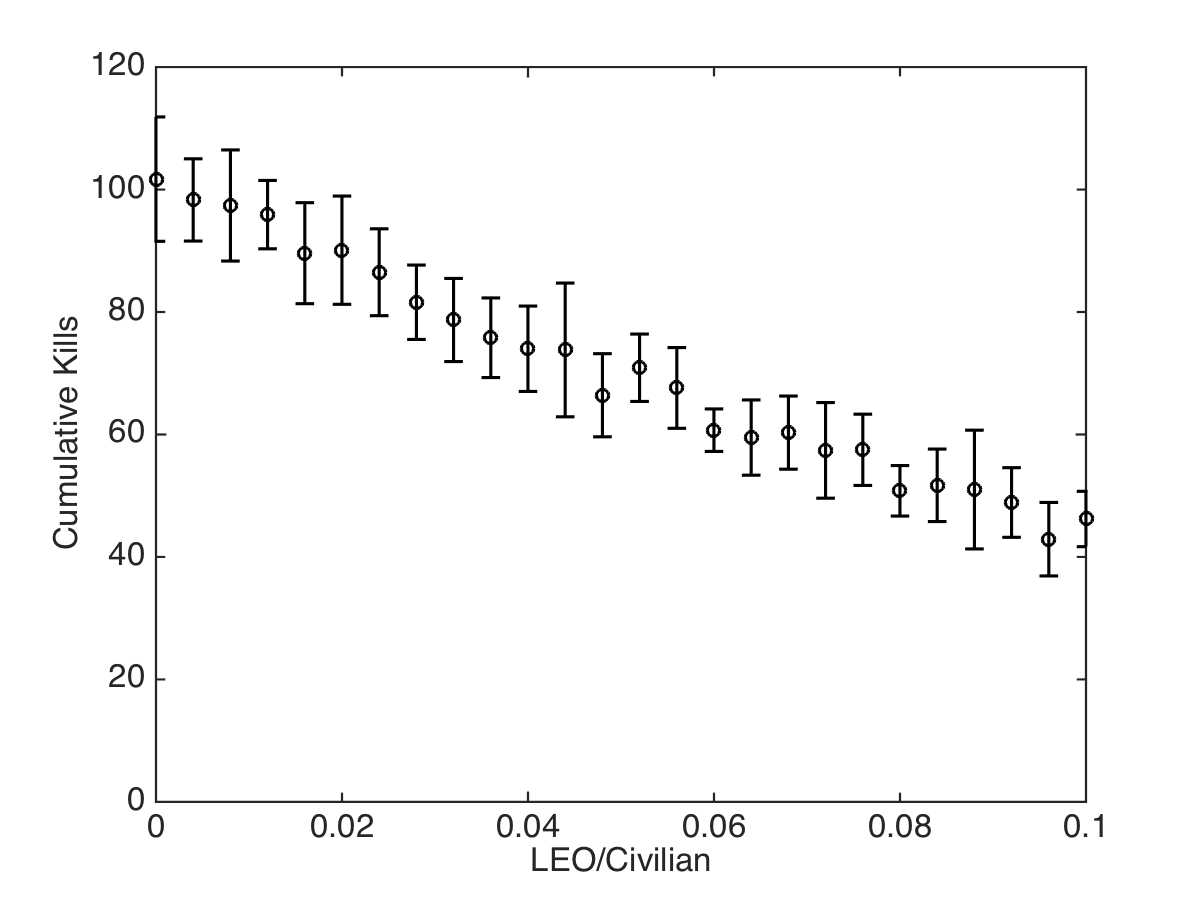
\includegraphics[width=0.80\textwidth]{../../code/modified_model/cum_kills_vs_LEO_civ.png}
	\caption{Effect of the initial LEO/civilian ratio on the cumulative number of kills at the end of the simulation using the modified model. Basically the same result as with the base model is obtained. Again, the mean formed out of 10 runs decreases with increasing LEO/civilian ratio. The standard deviation shown through remains fairly constant.}
	\label{fig:LEO_civ_modified}
\end{figure}

\subsubsection{Dependence on the Legitimacy and the Violence Threshold}
The results are shown in figures~\ref{fig:L_T_dep_base} and \ref{fig:L_T_dep_mod}. The (mean) violence threshold seems to have a larger impact on the extent of violence encountered during the simulation than the (mean) perceived legitimacy. Especially at low violence threshold values extreme extents of violence are encountered. This can be rationalized by recalling the criterion for a civilian to become active $(G-N)>T$. $G$ is approximately equal to $H$ when the perceived legitimacy is very high. $N$ is approximately equal to $R$ for the selected value of $k_P$. The mean difference $(H-R)$ is equal to zero, so for negative values of $T$/$\mu_T$., the civilians almost always become active, no matter what their surrounding looks like. The effect of the (mean) perceived legitimacy on the model output decreases with decreasing value of the (mean) violence threshold. This can be explained using the same arguments presented before. In the case of the modified model, the results are qualitatively identical to those of the base model. The variation in the individual values of $L$ and $T$ introduces especially some deviations for moderate values of $\mu_T$ and high values of $\mu_L$. Because there is a certain fraction of the population that has lower values of $L$ and $T$ than the mean, there will be more violence compared to the base models, where all civilians are identical regarding these characteristics.
\begin{figure}[!htbp]
	\centering
		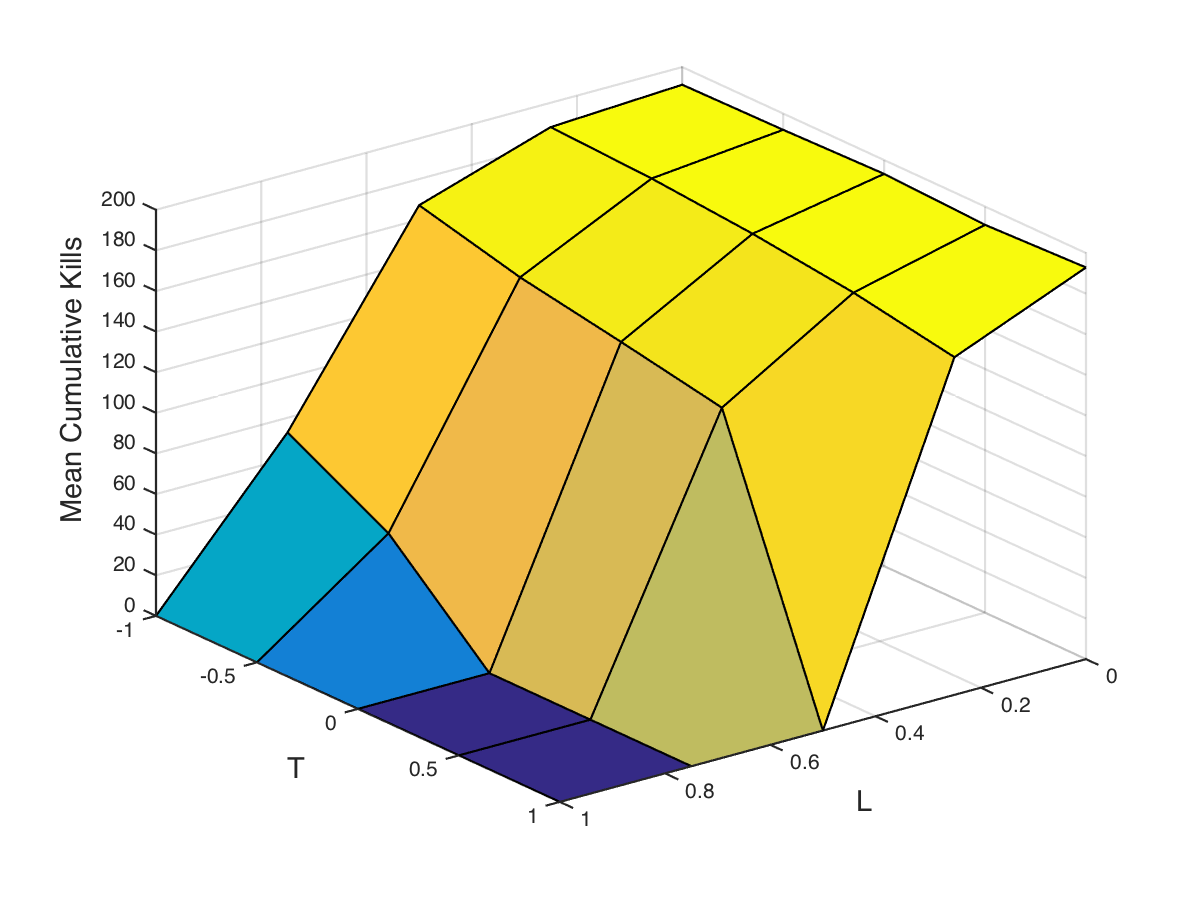
\includegraphics[width=0.80\textwidth]{../../code/base_model/L_T_dep_mean.png}
	\caption{Dependence of the mean cumulative number of kills on the two parameters $L$ and $T$ of the base model. The parameter $L$ seems to be more influential than $T$ for the selected values of the other model parameters.}
	\label{fig:L_T_dep_base}
\end{figure}
\begin{figure}[!htbp]
	\centering
		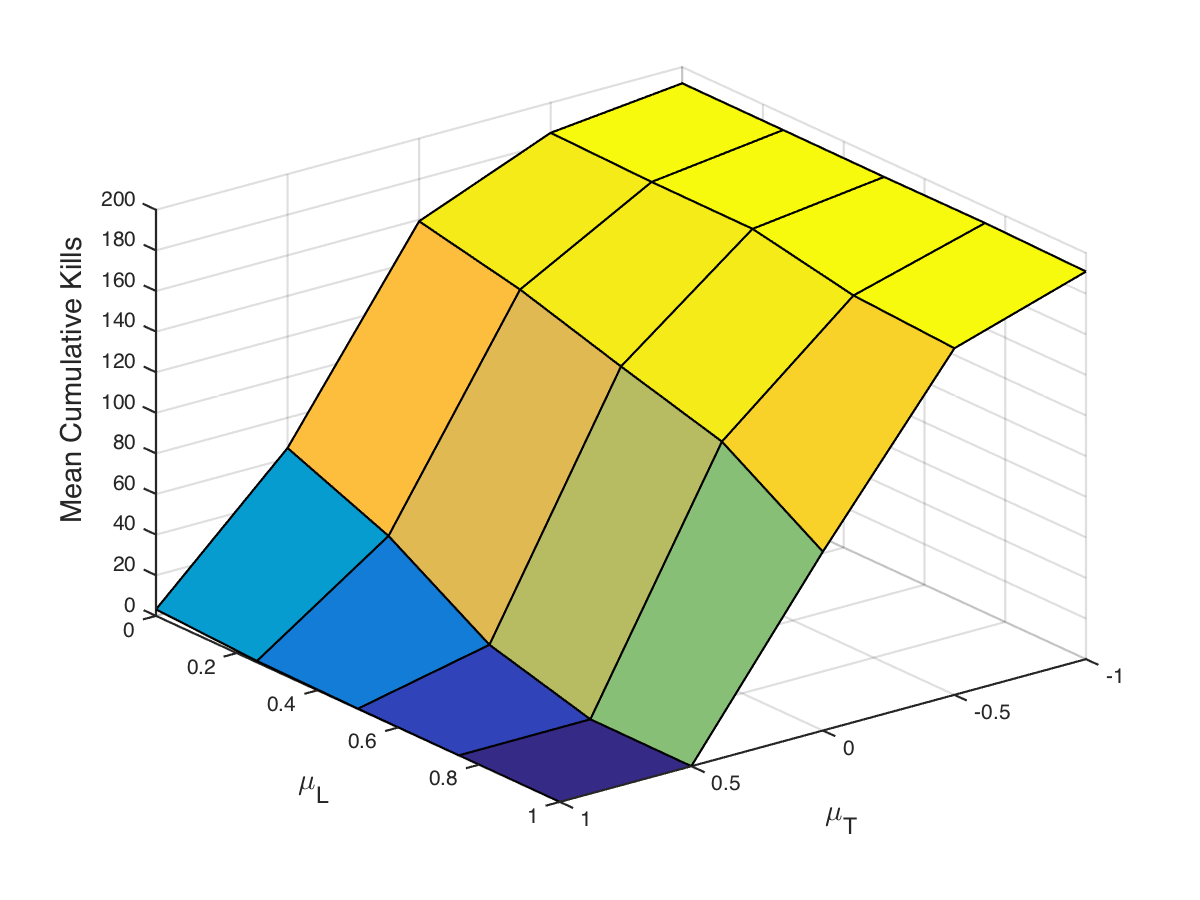
\includegraphics[width=0.80\textwidth]{../../code/modified_model/L_T_mean_dep_mean.png}
	\caption{Dependence of the mean cumulative number of kills on the two parameters $\mu_L$ and $\mu_T$ of the modified model. As in the base model, the output shows more sensitivity towards the parameter $L$ than the parameter $T$ for the selected values of the other model parameters.}
	\label{fig:L_T_dep_mod}
\end{figure}

\subsubsection{Dependence on the Parameters $\sigma_L$ and $\sigma_T$}
The results of this analysis are shown in figure~\ref{fig:L_T_std_dep}. The mean number of cumulative kills increases with increasing value of the standard deviations $\sigma_L$ and $\sigma_T$. This is most probable due to the increase in the number of extreme individuals on the map, which have low values of $L$ and/or $T$, although the means of those characteristics over the entire population remain unchanged. Those extreme individuals will very often engage in violence when they are selected. Therefore it would be important to not only have high mean perceived legitimacy and violence threshold, but also to have a homogeneous society regarding those characteristics in order to prevent extensive violence.
\begin{figure}[!htbp]
	\centering
		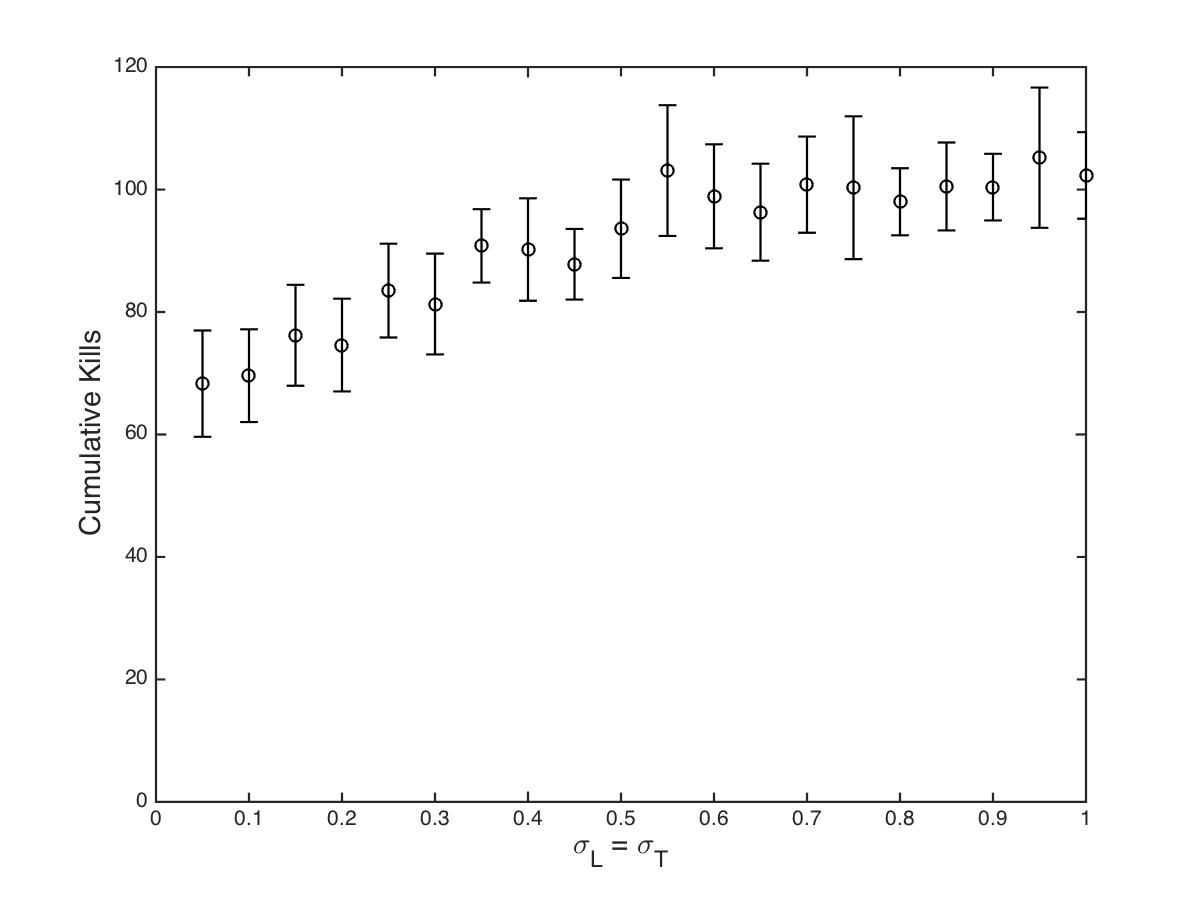
\includegraphics[width=0.80\textwidth]{../../code/modified_model/L_T_std_dep.png}
	\caption{Dependence of the mean cumulative number of kills on the value of the standard deviations $\sigma_L$ and $\sigma_T$ of the truncated normal distributions from which the two individual characteristics $L$ and $T$ of the civilians are drawn in the case of the modified model.}
	\label{fig:L_T_std_dep}
\end{figure}

\subsubsection{Dependence on the Parameter $k_L$}
The results are shown in figure~\ref{fig:k_L_dep}. As it can be seen, the parameter value seems to have almost no effect on the extent of violence encountered in the simulation. Based on the form of the equations~\eqref{eqn:update_violence} and \eqref{eqn:update_arrest}, one would expect an increase of the violence with increasing value of the parameter $k_L$. Kills have a stronger influence on the perceived legitimacy than arrests. Also are kills more likely to occur in the simulation because of the fewer selections of a LEO. That this was not observed might be mainly due to the fact, that the legitimacy is only updated in a rather short range around the killed/arrested civilian. Extending the range might increase the effect on the cumulative number of kills. It might make the model even more realistic, if the values of the constants $k_L$ in the two update equations can be different (increasing the relative effect of an arrest).
\begin{figure}[!htbp]
	\centering
		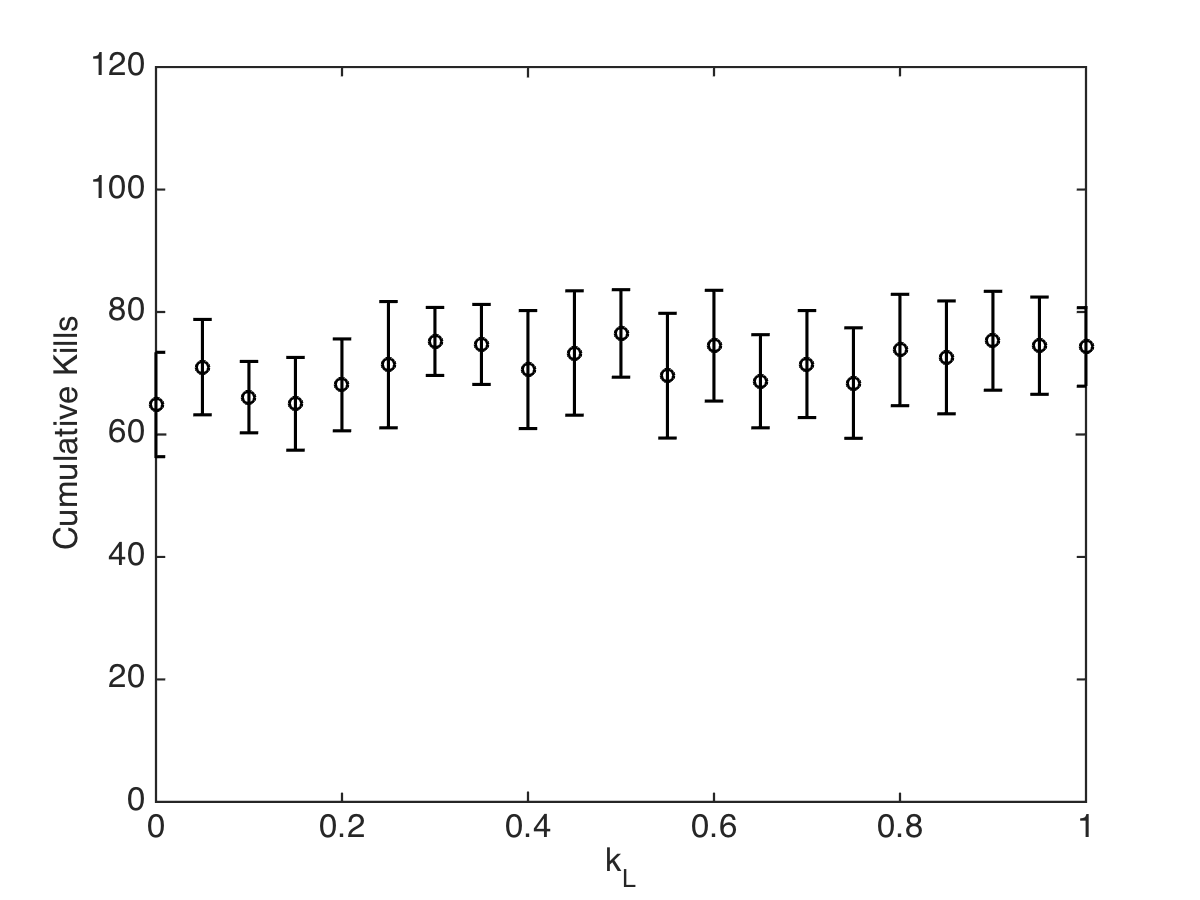
\includegraphics[width=0.80\textwidth]{../../code/modified_model/k_L_dep.png}
	\caption{Dependence of the mean cumulative number of kills on the value of the parameter $k_L$.}
	\label{fig:k_L_dep}
\end{figure}

\section{Summary and Outlook}
The base model presented in literature was extended by making the characteristics $L$ and $T$ of the civilians individual quantities. This was achieved by drawing them from a truncated normal distribution upon initialization of the civilians on the map. The normal distribution was selected instead of a uniform distribution because it seemed not to be realistic, that those quantities are uniformly distributed. This introduced four new parameters to the model: $\mu_L$, $\sigma_L$, $\mu_T$ and $\sigma_T$, removing the parameters $L$ and $T$. Further, a new interaction was introduced: the updating of the perceived legitimacy upon murders or arrests. This yielded another parameter $k_L$ used to describe this update. The next step could be to also change the distributions from which the other individual quantities (the hardship $H$ and the risk aversion $R$)) are drawn to a truncated normal distribution. Them being uniformly distributed over the population also seems to be not very realistic. Maybe the assumption that violence has always the same effect on the perceived legitimacy is too strong. It could be tried to use a formula similar to equation~\eqref{eqn:update_arrest} to describe the update of the legitimacy, but to use two different constants in the updating formulas.\\
\\
It was tried to assess the sensitivity of the model output to the various input parameters using a variance-based global sensitivity analysis method. As model output, the cumulative number of kills encountered over the course of the simulation normalized to the initial population size was defined. The application of this method failed due to unidentified reasons. One possible explanation would be an insufficient size of sample points. Increasing the sample size was not an option due to the lack of computational resources. This could for instance be overcome by using a computer cluster, since the computation of model outputs is tailor-made for parallelization. Also the number of iterations to generate the single model outputs could be increase, to better assess the evolution of the simulation and to consider long term effects inside the model.\\
\\
Lacking the results from the global sensitivity analysis, a more basic approach was made to evaluate the dependence of the extent of violence in the artificial society on some of the model parameters. First, it was tried to reproduce the findings from the literature regarding perceived legitimacy and LEO density. As in the reference, no violence was observed in the base model when the perceived legitimacy was as high as 0.9. In the modified model, there was always some violence due to the heterogeneity of the parameters $L$ and $T$. This seems to be a reasonable result. Even in the most peaceful, multi-cultural societies, racist violence occurs from time to time. The effect of the LEO density on the mean extent of violence was corresponding to that reported in literature. However, no increase in the standard deviation could be observed, but this is most probably attributed to the different method to measure the extent of violence compared to the reference.\\
\\
Both for the base and the modified model, the (mean) violence threshold was found to be more influential on the model output than the (mean) perceived legitimacy. This can be explained by the criterion for the selected civilian to become active or to stay quiet. The modified model showed generally more violence over the whole range of combinations of the mean perceived legitimacy and the mean violence threshold. This can be rationalized by the small probability to also have extreme individuals in the population.\\
\\
The parameter $k_L$ seems to have not a significant effect on the extent of violence encountered in the simulation. This might be due to limited range in which the update of the perceived legitimacy takes place. As next step, this range could be extended and the dependence of the model output on the value of the parameter $k_L$ could be reevaluated.

\section{References}






\end{document}  



 
